%2multibyte Version: 5.50.0.2960 CodePage: 1252
%\usepackage{mathpazo}


\documentclass[smaller]{beamer}\usepackage[]{graphicx}\usepackage[]{color}
% maxwidth is the original width if it is less than linewidth
% otherwise use linewidth (to make sure the graphics do not exceed the margin)
\makeatletter
\def\maxwidth{ %
  \ifdim\Gin@nat@width>\linewidth
    \linewidth
  \else
    \Gin@nat@width
  \fi
}
\makeatother

\definecolor{fgcolor}{rgb}{0.345, 0.345, 0.345}
\newcommand{\hlnum}[1]{\textcolor[rgb]{0.686,0.059,0.569}{#1}}%
\newcommand{\hlstr}[1]{\textcolor[rgb]{0.192,0.494,0.8}{#1}}%
\newcommand{\hlcom}[1]{\textcolor[rgb]{0.678,0.584,0.686}{\textit{#1}}}%
\newcommand{\hlopt}[1]{\textcolor[rgb]{0,0,0}{#1}}%
\newcommand{\hlstd}[1]{\textcolor[rgb]{0.345,0.345,0.345}{#1}}%
\newcommand{\hlkwa}[1]{\textcolor[rgb]{0.161,0.373,0.58}{\textbf{#1}}}%
\newcommand{\hlkwb}[1]{\textcolor[rgb]{0.69,0.353,0.396}{#1}}%
\newcommand{\hlkwc}[1]{\textcolor[rgb]{0.333,0.667,0.333}{#1}}%
\newcommand{\hlkwd}[1]{\textcolor[rgb]{0.737,0.353,0.396}{\textbf{#1}}}%
\let\hlipl\hlkwb

\usepackage{framed}
\makeatletter
\newenvironment{kframe}{%
 \def\at@end@of@kframe{}%
 \ifinner\ifhmode%
  \def\at@end@of@kframe{\end{minipage}}%
  \begin{minipage}{\columnwidth}%
 \fi\fi%
 \def\FrameCommand##1{\hskip\@totalleftmargin \hskip-\fboxsep
 \colorbox{shadecolor}{##1}\hskip-\fboxsep
     % There is no \\@totalrightmargin, so:
     \hskip-\linewidth \hskip-\@totalleftmargin \hskip\columnwidth}%
 \MakeFramed {\advance\hsize-\width
   \@totalleftmargin\z@ \linewidth\hsize
   \@setminipage}}%
 {\par\unskip\endMakeFramed%
 \at@end@of@kframe}
\makeatother

\definecolor{shadecolor}{rgb}{.97, .97, .97}
\definecolor{messagecolor}{rgb}{0, 0, 0}
\definecolor{warningcolor}{rgb}{1, 0, 1}
\definecolor{errorcolor}{rgb}{1, 0, 0}
\newenvironment{knitrout}{}{} % an empty environment to be redefined in TeX

\usepackage{alltt}
%%%%%%%%%%%%%%%%%%%%%%%%%%%%%%%%%%%%%%%%%%%%%%%%%%%%%%%%%%%%%%%%%%%%%%%%%%%%%%%%%%%%%%%%%%%%%%%%%%%%%%%%%%%%%%%%%%%%%%%%%%%%%%%%%%%%%%%%%%%%%%%%%%%%%%%%%%%%%%%%%%%%%%%%%%%%%%%%%%%%%%%%%%%%%%%%%%%%%%%%%%%%%%%%%%%%%%%%%%%%%%%%%%%%%%%%%%%%%%%%%%%%%%%%%%%%
\usepackage{amssymb}
\usepackage{amsmath}
\usepackage{graphicx}
\usepackage{hyperref}
\usepackage{multimedia}
\usepackage{epstopdf}
\usepackage{color}
\usepackage{tikz}


\setcounter{MaxMatrixCols}{10}
\newtheorem{remark}{Remark}[section]
\newtheorem{proposition}{Proposition}[section]
\newtheorem{interpretation}{Interpretation}[section]
\newtheorem{goal}{Goal}[section]
\newtheorem{statement}{Statement}[section]
\newtheorem{aes}{Aim \& Scope}[section]
\newtheorem{exercise}{Exercise}[section]
\renewcommand{\Pr}{P}

\newcommand{\mbf}[1]{\mathbf{#1}}
\newcommand{\beq}{\begin{equation}}
\newcommand{\eeq}{\end{equation}}
\newcommand{\bea}{\begin{eqnarray}}
\newcommand{\eea}{\end{eqnarray}}
\newcommand{\ba}{\begin{array}}
\newcommand{\ea}{\end{array}}
\newcommand{\bi}{\begin{itemize}}
\newcommand{\ei}{\end{itemize}}
\newcommand{\ben}{\begin{enumerate}}
\newcommand{\een}{\end{enumerate}}
\newcommand{\nn}{\nonumber}
\newcommand{\N}{\mathcal{N}}

\newenvironment{stepenumerate}{\begin{enumerate}[<+->]}{\end{enumerate}}
\newenvironment{stepitemize}{\begin{itemize}[<+->]}{\end{itemize} }
\newenvironment{stepenumeratewithalert}{\begin{enumerate}[<+-| alert@+>]}{\end{enumerate}}
\newenvironment{stepitemizewithalert}{\begin{itemize}[<+-| alert@+>]}{\end{itemize} }
\usetheme{Madrid}


%%%%%%%%%%%%%%%%%%%%%%%%%%%%%%%%%%%%%%%%%%%%%%%%%%%%%%%%%%%%%%%%%%%%%%%%%%%%%%%
% GSEM COLORS
%%%%%%%%%%%%%%%%%%%%%%%%%%%%%%%%%%%%%%%%%%%%%%%%%%%%%%%%%%%%%%%%%%%%%%%%%%%%%%%
\definecolor{darkGSEM}{RGB}{70,95,127}
\definecolor{darkGSEM2}{RGB}{40,80,150}
\definecolor{GSEM}{RGB}{96,121,153} % GSEM 10% lighter

%%% Global colors
\setbeamercolor*{palette primary}{use=structure,fg=white,bg=darkGSEM}
\setbeamercolor*{palette quaternary}{use=structure,fg=white,bg=darkGSEM!90}
\setbeamercolor{frametitle}{fg=white,bg=GSEM!80}

%%% TOC colors
\setbeamercolor{section in toc}{fg=darkGSEM}

%%% itemize colors
\setbeamertemplate{itemize items}[circle]
\setbeamercolor{itemize item}{fg=darkGSEM2}
\setbeamercolor{itemize subitem}{fg=darkGSEM2}
\setbeamercolor{itemize subsubitem}{fg=darkGSEM2}


%%% enumerate colors
\setbeamercolor{item projected}{fg=white,bg=GSEM}
\setbeamertemplate{enumerate item}{\insertenumlabel.}
\setbeamercolor{enumerate item}{fg=darkGSEM2}
\setbeamercolor{enumerate subitem}{fg=darkGSEM2}
\setbeamercolor{enumerate subsubitem}{fg=darkGSEM2}


\AtBeginSection[]
{
  \begin{frame}
    \frametitle{Outline}
    \tableofcontents[currentsection]
  \end{frame}
}

\AtBeginSubsection[]
{
  \begin{frame}
    \frametitle{Outline}
    \tableofcontents[currentsubsection]
  \end{frame}
}



%%%%%%%%%%%%%%%%%%%%%%%%%%%%%%%%%%%%%%%%%%%%%%%%%%%%%%%%%%%%%%%%%%%%%%%%%%%%%%%%
% R Chunk Options and Packages
%%%%%%%%%%%%%%%%%%%%%%%%%%%%%%%%%%%%%%%%%%%%%%%%%%%%%%%%%%%%%%%%%%%%%%%%%%%%%%%%




%%%%%%%%%%%%%%%%%%%%%%%%%%%%%%%%%%%%%%%%%%%%%%%%%%%%%%%%%%%%%%%%%%%%%%%%%%%%%%%%
\IfFileExists{upquote.sty}{\usepackage{upquote}}{}
\begin{document}

\title[S110015]{Probability 1}
\subtitle{Chapter 05 : Continuous Random Variables - Part 1}
\author[Flores-Agreda, La Vecchia]{Dr. Daniel Flores-Agreda, \\[0.5em] \tiny{(based on the notes of Prof. Davide La Vecchia)}}
\date{Spring Semester 2021}

\begin{frame}
\titlepage
\end{frame}


\begin{frame}{Objectives}

\begin{itemize}
\item Present the Exponential distribution \bigskip
\item Understand the consequences of the transformation of Random Variables.
\end{itemize}

\end{frame}

\begin{frame}{Outline}
\tableofcontents
\end{frame}

%%%%%%%%%%%%%%%%%%%%%%%%%%%%%%%%%%%%%%%%%%%%%%%%%%%%%%%%%%%%%%%%%%%%%%%%%%%%%%%%
\section{Exponential distribution}
%%%%%%%%%%%%%%%%%%%%%%%%%%%%%%%%%%%%%%%%%%%%%%%%%%%%%%%%%%%%%%%%%%%%%%%%%%%%%%%%

\begin{frame}{\secname}
  \begin{definition}
  Let $X$ be a  continuous random variable, having the following  characteristics:
  \begin{itemize}
  \item $X$ is defined on the \textbf{positive real numbers} $\left( 0;\infty \right)$ i.e. $\mathbb{R}^+$;
  \item the PDF and CDF are
  \bea
  f_X(x)=\lambda \exp\{ -\lambda x\},\lambda
  >0; &
  F_X(x)=1-\exp (-\lambda x); \nn \eea
  \end{itemize}
  then we say that $X$ has an \textbf{exponential distribution}.\bigskip

  We write $X\sim$ \text{Exp$(\lambda)$}.
  \end{definition}
\end{frame}

\begin{frame}{\secname}
  \begin{remark}[Expectation and Variance]
    For $X\sim$ \text{Exp$(\lambda)$} we have that:
    \begin{small}
    \bea
    E[X]= \frac{1}{\lambda} & \text{ and } &   Var(X)=\frac{1}{\lambda^{2}}.
    \eea
    \end{small}
  \end{remark}
  \pause

  \begin{remark}[Applications and Properties]
    $X$ is typically applied to model \textbf{the time until an event occurs}, when events are always occurring at a  rate $\lambda >0$. \bigskip

    \bigskip

    \bigskip

    \bigskip

    \bigskip


    The \textbf{sum of independent exponential} random variables has a \textbf{Gamma distribution} (see the exercises).
  \end{remark}
\end{frame}

\begin{frame}{\secname}
  \begin{example}[A graphical illustration]
  % \begin{figure}[ptb]\centering
  % 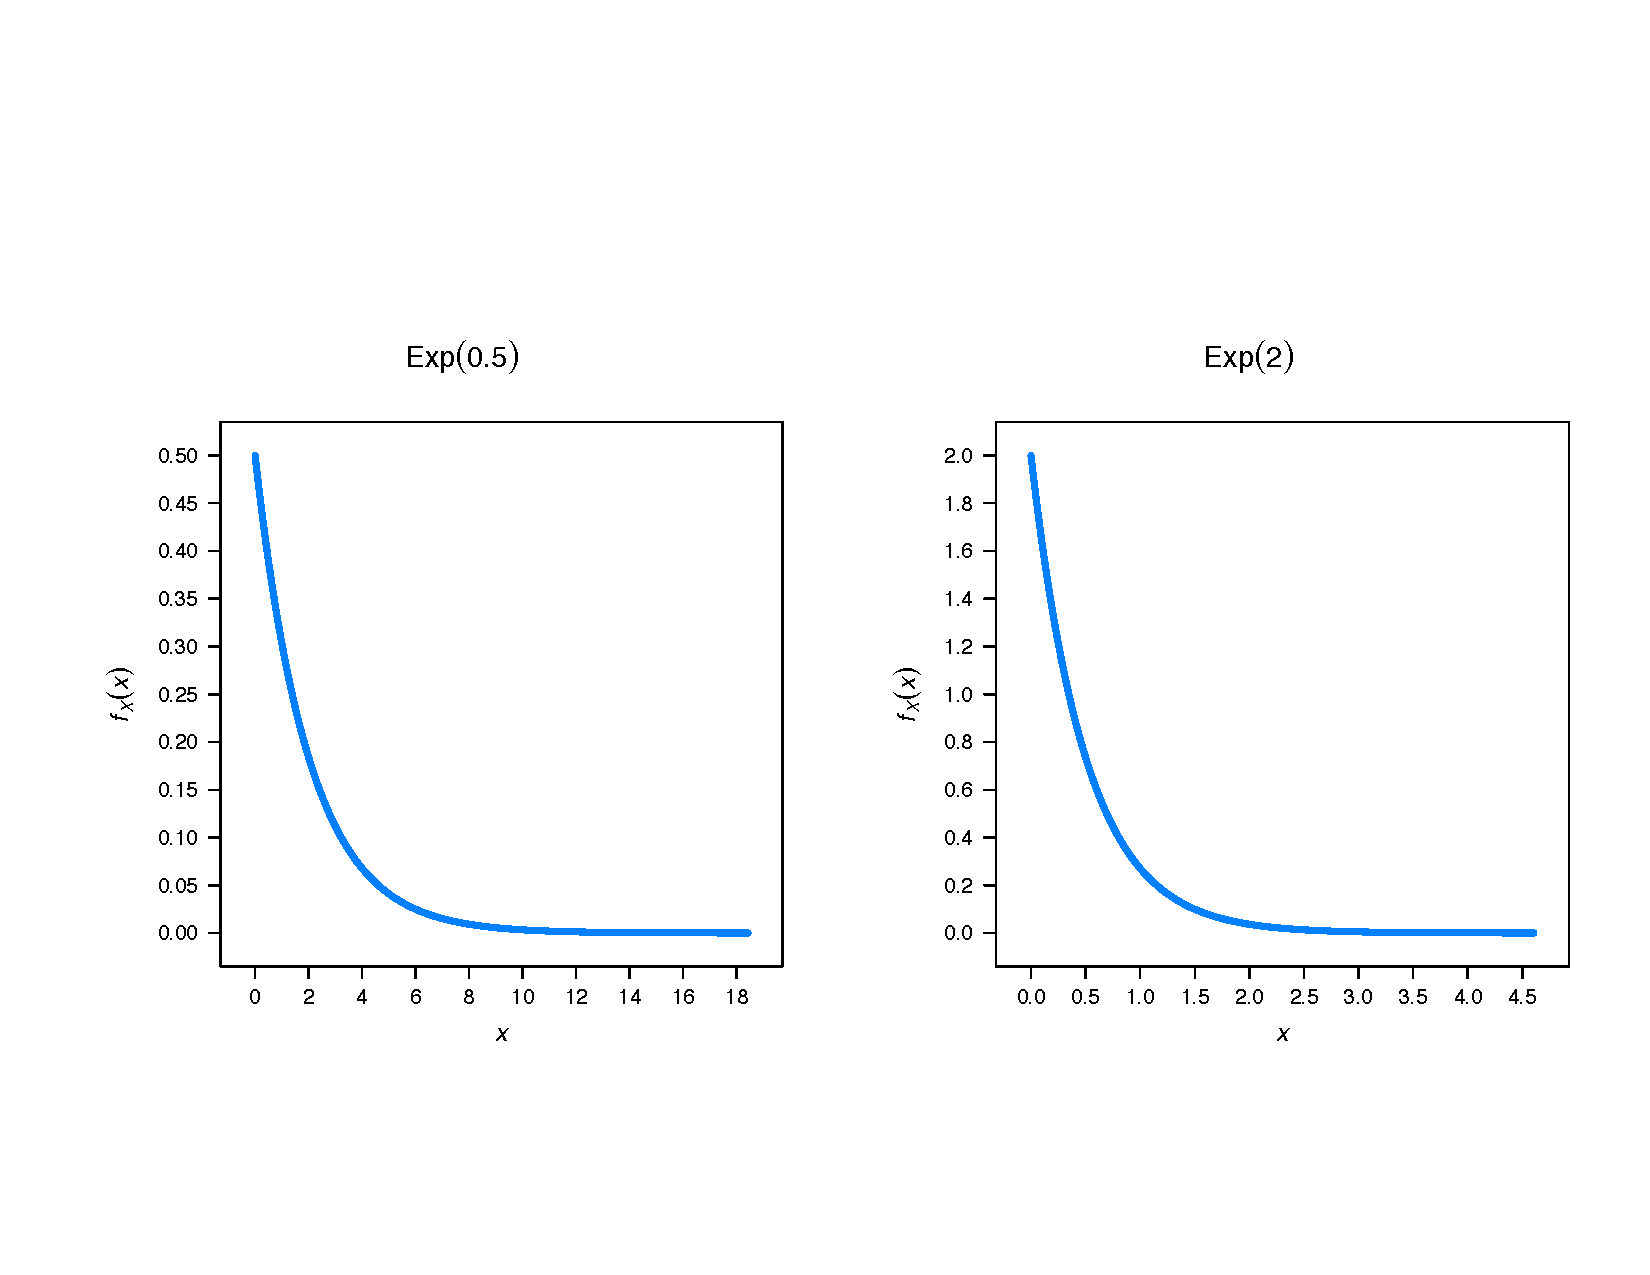
\includegraphics[height=2.4856in, width=4.5in]{img/Exp_Diego.pdf}%
  % \end{figure}
\begin{knitrout}
\definecolor{shadecolor}{rgb}{0.969, 0.969, 0.969}\color{fgcolor}

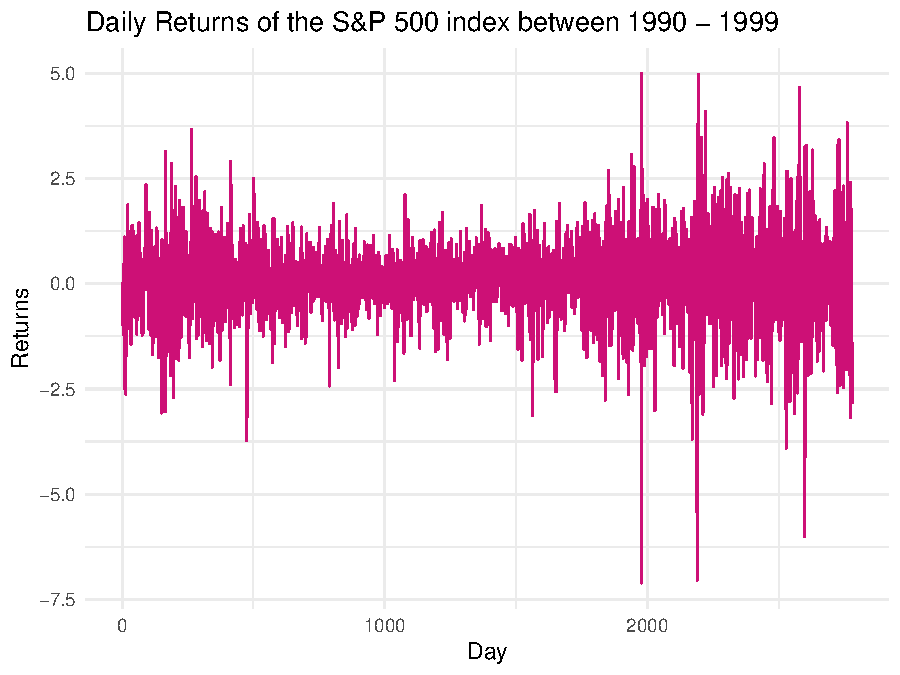
\includegraphics[width=0.5\linewidth]{figure/unnamed-chunk-2-1} \hfill{}



\end{knitrout}
  \end{example}
\end{frame}

\begin{frame}{\secname}
  \begin{example}[Illustration of use (Spoiler of the Exercises!)]
  \begin{footnotesize}
    The lifetime $X$ in years of a television follows an exponential law with density:
    \begin{equation*}
    f(x)=\lambda e^{-\lambda x} ,\quad x\geq 0.
    \end{equation*}
    \begin{enumerate}
      \item Compute the cumulative distribution function $F(x)$.
      \item Compute the $\alpha$-quantile $q_\alpha=F^{-1}(\alpha)$.
      \item The expected life of your television is $8$ years. What is the probability that the lifetime of your television is more than $8$ years ?
      Evaluate the median.
      \item Compute the variance of $X$ for any $\lambda$.
    \end{enumerate}
  \end{footnotesize}
  \end{example}
\end{frame}


\begin{frame}{\secname}

Unlike the Normal, the CDF of an exponential has a closed-form expression

  \begin{example}[CDF of Exponential]
  \begin{footnotesize}

  Let $X\sim$ \text{Exp}$(\lambda)$, with $\lambda =0.5$. Thus
  $$f_X(x) = \left\{ \begin{array}{ll}
  0.5 \exp (-0.5x) & x>0\\
  0 & \text{otherwise}
  \end{array} \right.$$
  Then, find the CDF.
  \pause

  \medskip

  For $x>0$, we have
  \begin{eqnarray*}
  F_{X}(x) & = & \int_{0}^{x}f_{X}(u)du\\
  & = & 0.5\Big( -2\exp (-0.5u)\Big) \bigl|_{u=0}^{u=x}\\
  & = & 0.5(-2\exp (-0.5x)+2\exp (0))\\
  & = & 1-\exp (-0.5x)
  \end{eqnarray*}
  \pause
  so, finally,

  $$F_X(x) = \left\{ \begin{array}{ll}
  0 & x \leq 0 \\
  1-\exp (-0.5x)& x>0
  \end{array} \right.$$
  \end{footnotesize}
  \end{example}
\end{frame}



%%%%%%%%%%%%%%%%%%%%%%%%%%%%%%%%%%%%%%%%%%%%%%%%%%%%%%%%%%%%%%%%%%%%%%%%%%%%%%%%
\section{Variable Transformation}
%%%%%%%%%%%%%%%%%%%%%%%%%%%%%%%%%%%%%%%%%%%%%%%%%%%%%%%%%%%%%%%%%%%%%%%%%%%%%%%%

\begin{frame}{\secname}
  \begin{remark}[Problem]
  Consider a random variable $X$ and suppose \textbf{we are interested in $Y=\psi(X)$}, where $\psi $ is a \textbf{
  \textbf{one to one} function}
  \end{remark}
  \pause
  \begin{definition}
  A \textbf{function }$\psi \left( x\right) $\textbf{\ is one to one}
  (1-to-1) if there are no two numbers, $x_{1},x_{2}$ in the domain of $\psi $
  such that $\psi \left( x_{1}\right) =\psi \left( x_{2}\right) $ but $%
  x_{1}\neq x_{2}$.
  \end{definition}
  \pause
  \begin{remark}
  A sufficient condition for $\psi \left( x\right) $ to be 1-to-1 is
  that it be monotonically increasing (or decreasing) in $x$.
  \bigskip
  \pause
  Note that the \textbf{inverse} of a 1-to-1 function $y=\psi \left(
  x\right) $ is a 1-to-1 function $\psi^{-1}\left( y\right) $ such that
  \begin{equation*}
  \psi ^{-1}\left( \psi \left( x\right) \right) =x\text{ and }\psi \left( \psi
  ^{-1}\left( y\right) \right) =y.
  \end{equation*}
  \end{remark}

  To transform $X$ to $Y$, we need to consider all the values $x$ that $X$ can take

  We first transform $x$ into values $y=\psi (x)$

\end{frame}

%%%%%%%%%%%%%%%%%%%%%%%%%%%%%%%%%%%%%%%%%%%%%%%%%%%%%%%%%%%%%%%%%%%%%%%%%%%%%%%%
\subsection{Transformation of Discrete Random Variables}
%%%%%%%%%%%%%%%%%%%%%%%%%%%%%%%%%%%%%%%%%%%%%%%%%%%%%%%%%%%%%%%%%%%%%%%%%%%%%%%%

\begin{frame}{\secname}
\framesubtitle{\subsecname}

  \begin{stepitemize}
  \item To transform a discrete random variable $X$, into the random variable $%
  Y=\psi (X)$, we transfer the probabilities for\textbf{\ each} $x$ to the values $%
  y=\psi \left( x\right) $:
  \begin{equation*}
  \begin{tabular}{l|cll|c}
  \multicolumn{2}{l}{\emph{Probability function for }$X$} &  &
  \multicolumn{2}{l}{\emph{Probability function for }$X$} \\
  &  &  &  &  \\
  $X$ & $\Pr \left(\{ X=x_{i} \}\right) =p_{i}$ &  & $Y$ & $\Pr \left(\{
  X=x_{i}  \}\right) =p_{i}$ \\ \cline{1-2}\cline{4-5}
  $x_{1}$ & $p_{1}$ & $\qquad \Rightarrow \qquad $ & $\psi (x_{1})$ & $p_{1}$
  \\
  $x_{2}$ & $p_{2}$ &  & $\psi (x_{2})$ & $p_{2}$ \\
  $x_{3}$ & $p_{3}$ &  & $\psi (x_{3})$ & $p_{3}$ \\
  $\vdots $ & $\vdots $ &  & $\vdots $ & $\vdots $ \\
  $x_{n}$ & $p_{n}$ &  & $\psi (x_{n})$ & $p_{n}$%
  \end{tabular}%
  \end{equation*}

  \item Note that this is equivalent to applying the function $\psi \left(
  \cdot \right) $ inside the probability statements:%
  \begin{eqnarray*}
  \Pr \left( \{ X=x_{i}  \}\right) &=&\Pr \left(  \{\psi \left( X\right) =\psi \left(
  x_{i}\right)  \} \right) \\
  &=&\Pr \left( \{ Y=y_{i} \} \right) \\
  &=&p_{i}
  \end{eqnarray*}
  \end{stepitemize}
\end{frame}


\begin{frame}{\secname}
  \framesubtitle{\subsecname}
  \begin{example}[option pricing]
\begin{footnotesize}
  Let us imagine that we are tossing a balanced coin ($p=1/2$), and when we get a ``Head'' ($H$) the stock price moves up of a factor $u$, but when we get a ``Tail'' ($T$) the price moves down of a factor $d$. We denote the price at time $t_1$  by $S_1(H)=u S_0 $ if the toss results in head ($H$), and by $S_1(T)=d S_0 $  if it results in tail ($T$). After the second toss, the price will be one of:
  \begin{figure}[ptb]\centering
  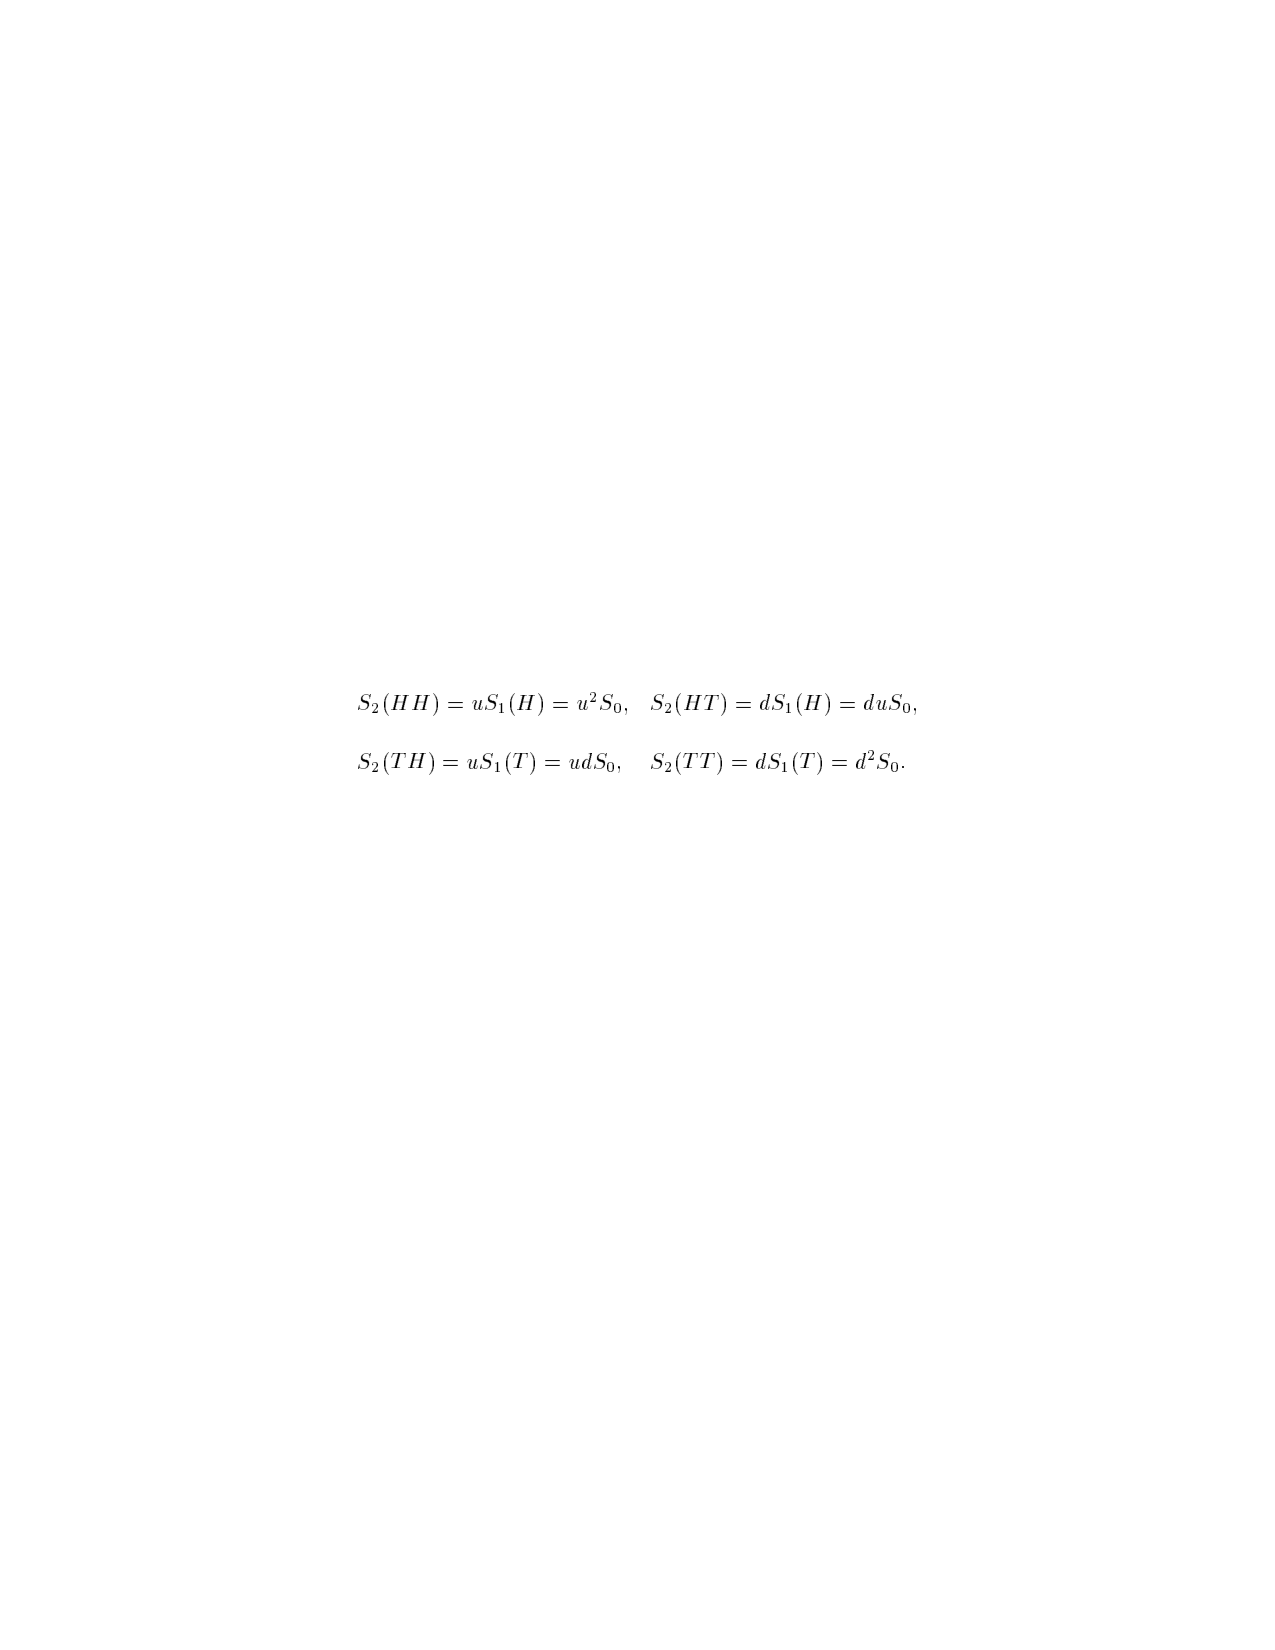
\includegraphics[height=0.75in, width=4in]{img/Shreve_Bin.pdf}%
  \end{figure}%
  Indeed, after two tosses, there are four possible coin sequences,
  $$
  \{HH,HT,TH,TT\}
  $$
  although not all of them result in different stock prices at time  $t_2$.
  %
  %% Define styles for bags and leafs
  %\tikzstyle{bag} = [text width=2em, text centered]
  %\tikzstyle{end} = []
  %\begin{tikzpicture}[sloped]
  %   \node (a) at ( 0,0) [bag] {$\$ A$};
  %   \node (b) at ( 4,-1.5) [bag] {B};
  %   \node (c) at ( 4,1.5) [bag] {C};
  %   \node (d) at ( 8,-3) [bag] {D};
  %   \node (e) at ( 8,0) [bag] {E};
  %   \node (f) at ( 8,3) [bag] {F};
  %   \draw [->] (a) to node [below] {$(1-p)$} (b);
  %   \draw [->] (a) to node [above] {$P$} (c);
  %   \draw [->] (c) to node [below] {$P^2$} (f);
  %   \draw [->] (c) to node [above] {$(1-p)p$} (e);
  %   \draw [->] (b) to node [below] {$(1-p)p$} (e);
  %   \draw [->] (b) to node [above] {$(1-p)^2$} (d);
  %\end{tikzpicture}
  \end{footnotesize}
  \end{example}
\end{frame}%

\begin{frame}{\secname}
  \framesubtitle{\subsecname}
  \begin{example}[continued]
  \begin{footnotesize}
  Let us set $S_0=1$, $u=2$ and $d=1/2$: we represent the price evolution by a tree:


  %
  %% Define styles for bags and leafs
  \tikzstyle{bag} = [text width=8em, text centered]
  \tikzstyle{end} = []
  \begin{tikzpicture}[sloped]
     \node (a) at ( 0,0) [bag] {$\$ 1$};
     \node (b) at ( 4,-1.5) [bag] {$\$ d =\$ 0.5$};
     \node (c) at ( 4,1.5) [bag] {$\$ u= \$ 2$};
     \node (d) at ( 8,-3) [bag] {$\$ d^2= \$ 0.25$};
     \node (e) at ( 8,0) [bag] {$\$ ud= \$ du = \$ 1$};
     \node (f) at ( 8,3) [bag] {$\$ u^2=\$ 4$};
     \draw [->] (a) to node [below] {$(1-p)$} (b);
     \draw [->] (a) to node [above] {$p$} (c);
     \draw [->] (c) to node [below] {$p^2$} (f);
     \draw [->] (c) to node [above] {$(1-p)p$} (e);
     \draw [->] (b) to node [below] {$(1-p)p$} (e);
     \draw [->] (b) to node [above] {$(1-p)^2$} (d);
  \end{tikzpicture}
  \end{footnotesize}
  \end{example}
\end{frame}

\begin{frame}{\secname}
\framesubtitle{\subsecname}
  \begin{example}[continued]
  Now consider an European option call with maturity $t_2$ and strike price $K=0.5$, whose random pay-off at $t_2$ is $C=\max(0;S_2-0.5)$. Thus,
  \begin{eqnarray*}
  C(HH)=\max(0;4-0.5)=\$ 3.5 & C(HT)=\max(0;1-0.5)=\$ 0.5 \\
  C(TH)=\max(0;1-0.5)=\$ 0.5 & C(TT)=\max(0;0.25-0.5)=\$ 0.
  \end{eqnarray*}
  Thus at maturity $t_2$ we have
  \begin{equation*}
  \begin{tabular}{l|cll|c}
  \multicolumn{2}{l}{\emph{Probability function for }$S_2$} &  &
  \multicolumn{2}{l}{\emph{Probability function for }$C$} \\
  &  &  &  &  \\
  $S_2$ & $\Pr \left(\{ X=x_{i} \}\right) =p_{i}$ &  & $C$ & $\Pr \left(\{
  C=c_{i}  \}\right) =p_{i}$ \\ \cline{1-2}\cline{4-5}
  $\$ u^2$ & $p^2$ & $\qquad \Rightarrow \qquad $ & $\$ 3.5$ & $p^2$
  \\
  $\$ ud$ & $2p(1-p)$ &  & $\$ 0.5$ & $2p(1-p)$ \\
  %$\$ du$ & $(1-p)p$ &  & $\$ 0.5$ & $(1-p)p$ \\
  $\$ d^2$ & $(1-p)^2$  &  & $\$ 0$ & $(1-p)^2$%
  \end{tabular}%
  \end{equation*}
  \tiny{Since $ud=du$ the corresponding values of $S_2$ and $C$ can be aggregated, without loss of info.}
  \end{example}
\end{frame}%

%%%%%%%%%%%%%%%%%%%%%%%%%%%%%%%%%%%%%%%%%%%%%%%%%%%%%%%%%%%%%%%%%%%%%%%%%%%%%%%%
\subsection{Transformation through the CDF}
%%%%%%%%%%%%%%%%%%%%%%%%%%%%%%%%%%%%%%%%%%%%%%%%%%%%%%%%%%%%%%%%%%%%%%%%%%%%%%%%

\begin{frame}{\secname}
\framesubtitle{\subsecname}

  \begin{stepitemize}
  \item We can use the same logic for CDF probabilities, whether the random
  variables are\textbf{\ discrete or continuous}

  \item Let $Y=\psi \left( X\right) $ with $\psi \left( x\right) $ \textbf{1-to-1 and
  monotone increasing}. Then
  \begin{eqnarray*}
  F_{Y}\left( y\right) &=&\Pr \left( \{ Y\leq y \}\right) \\
  &=&\Pr \left( \{ \psi \left( X\right) \leq y \} \right) =\Pr \left( \{ X\leq \psi
  ^{-1}\left( y\right) \} \right) \\
  &=&F_{X}\left( \psi ^{-1}\left( y\right) \right)
  \end{eqnarray*}

  \begin{example}
  Let $Y=\psi \left( X\right) =\exp{ X} $ where $%
  X\sim F_X$ on all values $x\in
  %TCIMACRO{\U{211d} }%
  %BeginExpansion
  \mathbb{R}
  %EndExpansion
  $%
  \begin{eqnarray*}
  F_{Y}\left( y\right) &=&\Pr \left( \{ Y\leq y \} \right) \\
  &=&\Pr \left( \{ \exp{  X} \leq y \} \right) =\Pr \left( \{ X\leq \ln
  \left( y\right) \} \right) \\
  &=&F_{X}\left( \ln \left( y\right) \right) \text{ only for }y>0\text{.}
  \end{eqnarray*}
  \end{example}

  %\item True whether $X$ (and hence $Y$) are continuous or discrete random
  %variables.
  \end{stepitemize}

  %TCIMACRO{\TeXButton{EndFrame}{\end{frame}}}%
  %BeginExpansion
\end{frame}%

\begin{frame}{\secname}
\framesubtitle{\subsecname}

  \begin{itemize}
  \item \textbf{Monotone decreasing functions} work in a similar way, but require
  \textbf{changing the sense of the inequality}.

  \item Let $Y=\psi \left( X\right) $ with $\psi \left( x\right) $ 1-to-1 and
  \textbf{monotone decreasing}. Then
  \begin{eqnarray*}
  F_{Y}\left( y\right) &=&\Pr \left( \{ Y\leq y \} \right) \\
  &=&\Pr \left( \{ \psi \left( X\right) \leq y \} \right) =\Pr \left( \{ X\geq \psi
  ^{-1}\left( y\right) \} \right) \\
  &=&1-F_{X}\left( \psi ^{-1}\left( y\right) \right)
  \end{eqnarray*}

  \end{itemize}

  \pause

  \begin{example}
  \begin{footnotesize}
  Example: let $Y=\psi \left( X\right) =-\exp X $ where $%
  X\sim F_X$ on all values $x\in
  %TCIMACRO{\U{211d} }%
  %BeginExpansion
  \mathbb{R}
  %EndExpansion
  $%
  \begin{eqnarray*}
  F_{Y}\left( y\right) &=&\Pr \left( \{ Y\leq y \}\right) =\Pr \left( \{ -\exp ^
  X \leq y \} \right) \\
  &=&\Pr \left( \{ \exp X \geq -y \} \right) =\Pr \left( \{ X\geq \ln
  \left( -y\right) \} \right) \\
  &=&1-F_{X}\left( \ln \left( -y\right) \right) \text{ only for }y<0\text{.}
  \end{eqnarray*}
  \end{footnotesize}
  \end{example}
\end{frame}

%%%%%%%%%%%%%%%%%%%%%%%%%%%%%%%%%%%%%%%%%%%%%%%%%%%%%%%%%%%%%%%%%%%%%%%%%%%%%%%%
\subsection{Transformation of Continuous Random Variables through the PDF}
%%%%%%%%%%%%%%%%%%%%%%%%%%%%%%%%%%%%%%%%%%%%%%%%%%%%%%%%%%%%%%%%%%%%%%%%%%%%%%%%

\begin{frame}{\secname}
  \framesubtitle{\subsecname}

  \begin{stepitemize}
  \item For continuous random variables, if $\psi \left( x\right) $ 1-to-1 and
  monotone \textbf{increasing}, we have%
  \begin{equation*}
  F_{Y}\left( y\right) =F_{X}\left( \psi ^{-1}\left( y\right) \right)
  \end{equation*}

  \item Notice this implies that the pdf of $Y=\psi \left( X\right) $ must
  satisfy%
  \begin{eqnarray*}
  f_{Y}\left( y\right) &=&\frac{dF_{Y}\left( y\right) }{dy}=\frac{dF_{X}\left(
  \psi ^{-1}\left( y\right) \right) }{dy} \\
  &=&\frac{dF_{X}\left( x\right) }{dx}\times \frac{d\psi ^{-1}\left( y\right)
  }{dy}\qquad \text{{\small (chain rule)}} \\
  &=&f_{X}\left( x\right) \times \frac{d\psi ^{-1}\left( y\right) }{dy}\qquad
  \text{{\small (derivative of CDF (of }}X\text{){\small \ is pdf)}} \\
  &=&f_{X}\left( \psi ^{-1}\left( y\right) \right) \times \frac{d\psi
  ^{-1}\left( y\right) }{dy}\qquad \text{{\small (substitute }}x=\psi
  ^{-1}\left( y\right) \text{{\small )}}
  \end{eqnarray*}
  \end{stepitemize}

\end{frame}

\begin{frame}{\secname}
  \framesubtitle{\subsecname}

  \begin{stepitemize}
  \item What happens when $\psi \left( x\right) $ 1-to-1 and monotone \textbf{%
  decreasing}? We have%
  \begin{equation*}
  F_{Y}\left( y\right) =1-F_{X}\left( \psi ^{-1}\left( y\right) \right)
  \end{equation*}

  \item So now the pdf of $Y=\phi \left( X\right) $ must satisfy
  \begin{eqnarray*}
  f_{Y}\left( y\right) &=&\frac{dF_{Y}\left( y\right) }{dy}=-\frac{%
  dF_{X}\left( \psi ^{-1}\left( y\right) \right) }{dy} \\
  &=&-f_{X}\left( \psi ^{-1}\left( y\right) \right) \times \frac{d\psi
  ^{-1}\left( y\right) }{dy}\qquad \text{{\small (same reasons as before)}}
  \end{eqnarray*}

  \item but $\frac{d\psi ^{-1}\left( y\right) }{dy}<0$ since here $\psi \left(
  \cdot \right) $ is monotone decreasing, hence we can write%
  \begin{equation*}
  f_{Y}\left( y\right) =f_{X}\left( \psi ^{-1}\left( y\right) \right) \times
  \left\vert \frac{d\psi ^{-1}\left( y\right) }{dy}\right\vert
  \end{equation*}

  \item This expression (called Jacobian-formula) is valid for $\psi \left( x\right) $ 1-to-1 and
  monotone (whether increasing or decreasing)
  \end{stepitemize}
\end{frame}

\begin{frame}{\secname}
  \framesubtitle{\subsecname}

  \begin{example}
  \begin{footnotesize}
  \begin{stepitemize}
  \item So what is the pdf for the lognormal distribution?

  \item Recall that $Y$ has a \textbf{lognormal distribution} when $\ln \left(
  Y\right) =X$ has a Normal distribution

  \item $\Rightarrow $ if $X\sim \N\left( \mu ,\sigma ^{2}\right) ,$ then $%
  Y=\exp X \sim $ \emph{lognormal}$\left( \mu ,\sigma ^{2}\right) $

  \begin{stepitemize}
  \item Corresponding to $\psi \left( x\right) =\exp x$ and $\psi
  ^{-1}\left( y\right) =\ln (y)$
  \end{stepitemize}

  \item The \emph{pdf} of $X$ is
  \begin{equation*}
  f_{X}\left( x\right) =\frac{1}{\sqrt{2\pi \sigma ^{2}}}\exp{ \left\{ -\frac{1%
  }{2\sigma ^{2}}\left( x-\mu \right) ^{2}\right\}}
  \end{equation*}%
  for any $-\infty <x<\infty $

  \item Using $\psi \left( x\right) =\exp x$ we know we'll have possible
  values for $Y$ only on $0<y<\infty $
  \end{stepitemize}
  \end{footnotesize}
  \end{example}
\end{frame}

\begin{frame}{\secname}
  \framesubtitle{\subsecname}
  \begin{example}[continued]
  \begin{footnotesize}
  \begin{stepitemize}
  \item We know that
  \begin{equation*}
  f_{Y}\left( y\right) =f_{X}\left( \psi ^{-1}\left( y\right) \right) \times
  \left\vert \frac{d\psi ^{-1}\left( y\right) }{dy}\right\vert
  \end{equation*}

  \item And since $\psi ^{-1}\left( y\right) =\ln (y)$ then
  \begin{equation*}
  \left\vert \frac{d\psi ^{-1}\left( y\right) }{dy}\right\vert =\left\vert
  \frac{1}{y}\right\vert
  \end{equation*}

  \item $\Rightarrow $ the \emph{pdf} of $Y$ is
  \begin{equation*}
  f_{Y}\left( y\right) =\frac{1}{y\sqrt{2\pi \sigma ^{2}}}\exp{ \left\{ -\frac{1%
  }{2\sigma ^{2}}\left( \ln (y)-\mu \right) ^{2}\right\}}
  \end{equation*}
  for any $0<y<\infty $
  \end{stepitemize}
  \end{footnotesize}
  \end{example}
\end{frame}

\begin{frame}{\secname}
\framesubtitle{\subsecname}
  \begin{example}[continued]
  \begin{footnotesize}
  \begin{stepitemize}
  \item Both the Normal and the lognormal are characterized by
  only two parameters ($\mu$ and $\sigma$). The \emph{median} of the lognormal distribution is $\exp{
  \mu } $, since $$
  \Pr \left( \{ X\leq \mu \} \right) = 0.5,
  $$
  and hence%
  \begin{eqnarray*}
  0.5 &=&\Pr \left(\{ X\leq \mu \}\right) \\
  &=&\Pr \left( \{\exp{X} \leq \exp{ \mu }\} \right) \\
  &=&\Pr \left( \{Y\leq \exp{ \mu }\} \right).
  \end{eqnarray*}
  \end{stepitemize}
  \end{footnotesize}
  \end{example}
  % More generally, for $\alpha\in[0,1]$, the $\alpha$-th quantile of a r.v. $X$ is the value $x_\alpha$ such that $P(\{X \leq x_\alpha\})\geq\alpha$. If $X$ si a continuous r.v.  we can set $P(\{X \leq x_\alpha\})=\alpha$ (as we did, e.g., for the lognormal).
\end{frame}

\begin{frame}{\secname}
\framesubtitle{A Word of Warning}

  When $X$ and $Y$ are two random variables, \textbf{we should pay attention to their transformations}. \medskip

  For instance, let us consider
  $$
  X\sim \mathcal{N}(\mu,\sigma^2) \quad \text{and}  \quad Y\sim Exp(\lambda).
  $$
  Then, let's transform $X$ and $Y$

  \begin{itemize}
  \item  in a linear way: $Z=X+Y$. We know that
  $$
  E[Z] = E[X+Y] = E[X] + E[Y]
  $$
  %so we can rely on the linearity of the expected value.
  \item in a nonlinear way $W = X/Y$. One can show that
  $$\color{red}
  E[W] = E\left[\frac{X}{Y}\right] \neq \frac{E[X]}{E[Y]}. \color{black}
  $$
  %so, we cannot rely on the linearity of the expected value.
   \end{itemize}
\end{frame}

\begin{frame}{{\secname}}
  \framesubtitle{The big picture}

  Despite exotic names, the common distributions relate to each other in intuitive and interesting ways. Several follow naturally from the Bernoulli distribution, for example.
\end{frame}


\begin{frame}{{\secname}}
  \framesubtitle{The big picture}

  \begin{figure}[ptb]\centering
  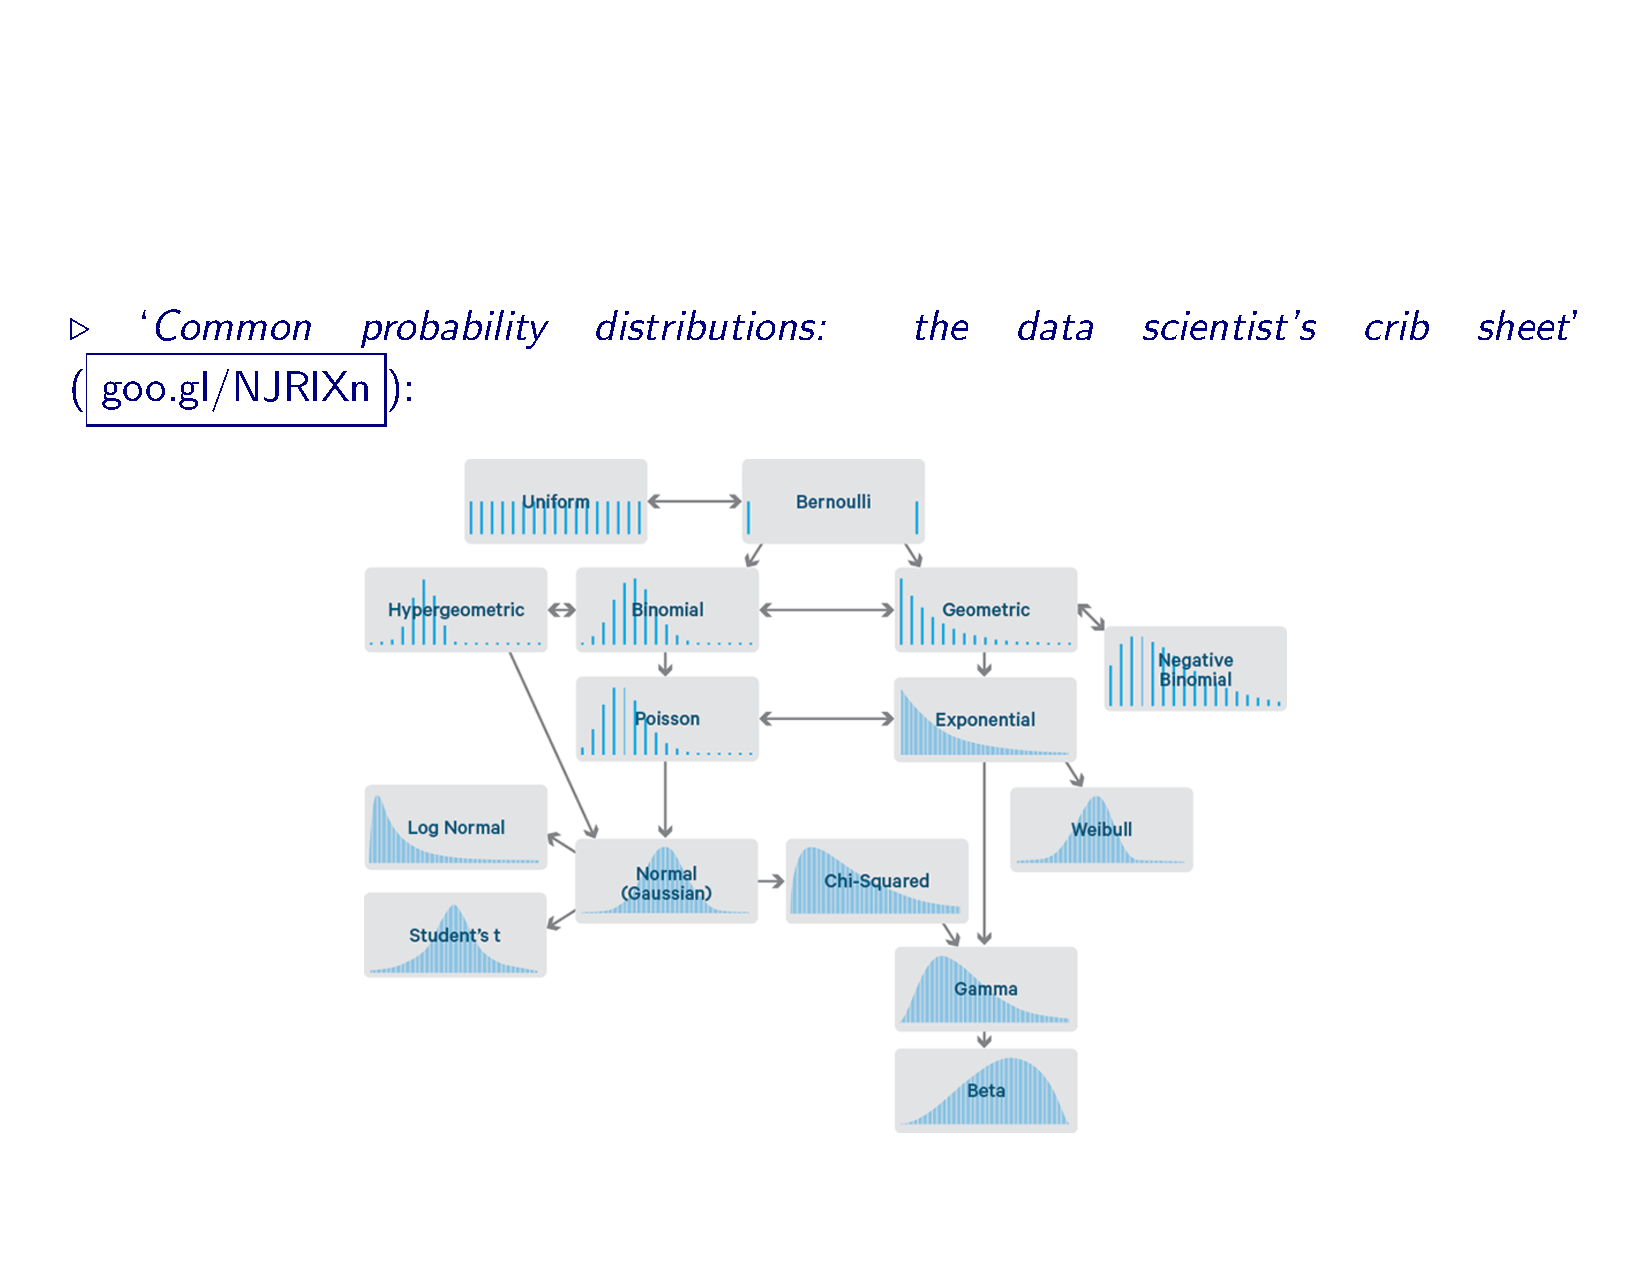
\includegraphics[scale = 0.45]{img/RelRVs_Diego.pdf}%
  \end{figure}
\end{frame}



\begin{frame}{Wrap-up}
  \begin{itemize}
  \item The Exponential distribution helps to model \emph{duration} data.\bigskip
  \item To compute the probabilities of transformed Discrete Random Variables we proceed on the Probability Function:
  $$P(X = x) = P(\psi(X) = \psi(x)) = P(Y = \psi(x))$$
  \item This principle applies to the inequalities in the CDF (give or take the sense of the monotonicity)
  \begin{align*}
  F_X(x) &= P(X \leq x) = P(\psi(X) \leq \psi(x)) = P(Y \leq \psi(x)) = F_Y(\psi(x)) \\
  F_X(x) &= P(X \leq x) = P(\psi(X) \geq \psi(x)) = P(Y \geq \psi(x)) = 1-F_Y(\psi(x))
  \end{align*}
  \item The density of a transformed variable can be found with the formula:
  \begin{equation*}
  f_{Y}\left( y\right) =f_{X}\left( \psi ^{-1}\left( y\right) \right) \times
  \left\vert \frac{d\psi ^{-1}\left( y\right) }{dy}\right\vert
  \end{equation*}
  \end{itemize}
\end{frame}

\begin{frame}
  \begin{center}
  \Large{Thank You for your Attention!}

  \bigskip
  \pause

  \Large{``See you'' Next Week}
  \end{center}
\end{frame}

\end{document}
